\section{Uvod}
\label{sec:uvod_id}
\setlength{\intextsep}{10pt}
\setcounter{equation}{0}
    ''Svaki dan na X je divan dan!'' - Elon Musk 2024. 
    Elon Musk je dodao polisu na platformi Tviter koja dopušta veštačkoj inteligenciji da uči kako da generiše od bilo kojih slika. To takođe uključuje umetnike i njihova dela koja su postavljena na platformi. Zatim je postavio sliku čime je hteo da pokaže kako VI može da "nauči i kreira umetnost". 


    \begin{wrapfigure}[13]{l}{0.4\textwidth}
    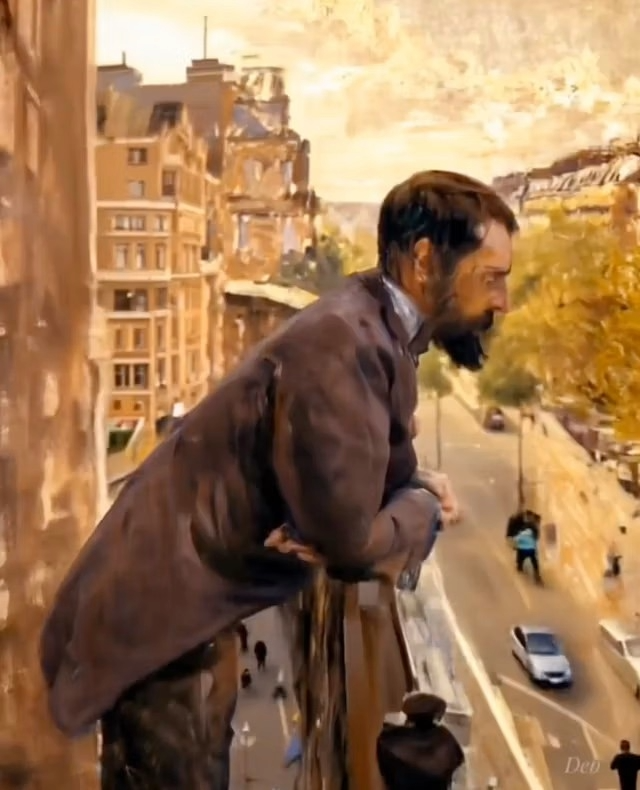
\includegraphics[width=0.38\textwidth]{Pictures/crtez.png}
    \end{wrapfigure}

    Kao što možemo da vidimo, na ovoj slici se svakakve stvari desavaju. Čovek bi trebalo da stoji na terasi, ali ovde vidimo da lebdi u vazduhu dok ljudi ispod njega šetaju. Ljudi voze moderne automobile i ljudi takođe šetaju po ulici. Na pozicijama gde bi trebalo prozori da budu su samo dizorijentisane mrljotine.

    Elon Muskova slika predstavlja VI mešavinu Kubertove \textit{Očajnik} (Le Désespéré) (1843-45) i Kajbotovog \textit{Čoveka na balkonu} (Man on the Balcony) (1880). Kao što se da primetiti, kola iz 21. veka nisu postojala u momentu kada su ovi crteži bili napravljeni iako su ''nacrtani'' na slici. \cite{musk_ai_art_2024} 

    \par
    \vspace{1cm}
    Pre nego što uopšte možemo da kritikujemo kako je ova slika napravljena, potrebno je da se zapitamo kakav je proces kreiranja slike preko veštačke inteligencije.

\subsection{Šta je veštačka inteligencija?}
    Teško je definisati šta je veštačka inteligencija sama po sebi. Alan Tjuring je u svojoj skripti 
    ''Computing machinery and intelligence'' rekao da se mašina može proglasiti pametnom ukoliko je nemoguće razaznati razliku između nje i čoveka u toku razgovora sa nekim slučajno izabranim posmatračem. \cite{turing2007computing} U današnje vreme bismo mogli reći da je mašina pametna ukoliko može da govori, razmišlja i postupa na sličan način kao što bi čovek uradio.
     
    
    Dosta novih inicijativa kreće iz same teme kako AI može da napravi umetnost, ali razumevanje i uvažavanje toga šta je umetnost može samo čovek da potvrdi. Potrebno je postaviti pitanje kako je moguće da mašina nauči kako da kreira nešto poput umetnosti kao čovek. Da bismo odgovorili na to pitanje, potrebno je ukratko objasniti kako AI vidi crteže. 

    Masovna digitalizacija slika i umetnosti u poslednjih nekoliko godina je omogućila njihovu dostupnost na internetu. Pored toga imamo i digitalnu umetnost koja takođe predstavlja novu skup podataka koje je neophodno istražiti. Fizikalna i digitalna slika postoje u različitim materijalnim oblastima, ali pokazuju istu složenu strukturu podataka koja opisuje tu sliku. Kao što svaki potez četkice na slici ima svoju ulogu, tako i svaki broj u njenoj numeričkoj reprezentaciji ima poentcijal koji treba istražiti. Bitno je naglasiti da ćemo nad tim numeričkim reprezentacijama primeniti različite naprednije algoritme kojim otvaramo novu prespektivu o samoj digitalizovanoj slici.

    \begin{figure}[H]
        \centering
        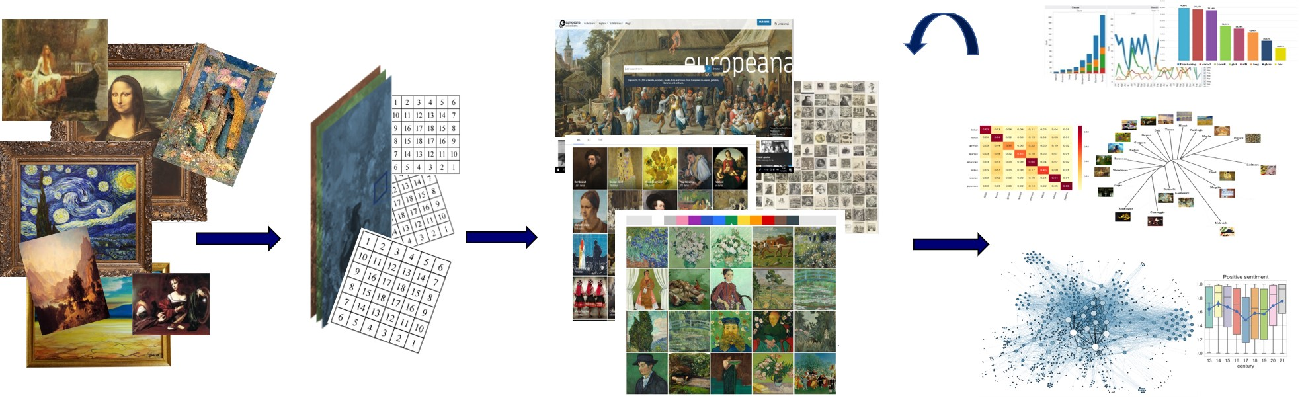
\includegraphics[width=1.0\linewidth]{Pictures/2-Figure1-1.png}
        \caption{Proces digitalizacije podataka}
    \end{figure}

    Gornja slika ilustruje proces od digitalizacije do kvantitativne analize, otkrivanja znanja i vizuelizacije korišćenjem računarskih metoda. Rezultati istraživanja dobijeni iz završne faze ovog procesa često se koriste za poboljšanje funkcionalnosti repozitorijuma i onlajn kolekcija dodavanjem naprednih načina istraživanja sadržaja.

\subsection{Koraci za treniranje veštačke inteligencije}
    Pošto su slike postale digitalizovane i sada predstavljaju vrstu podataka, potrebno je da uradimo sledeći korak, što je klasifikacija. Tokom poslednje decenije, najbitniji izazov je bio automatizovati klasifikaciju umetničkih dela na osnovu kategorija kao što su umetnik, stil i žanr. Koršićenjem konvolutnih neuronskih mreža, dobijen je ogroman napredak u poboljšanju tačnosti klasifikacije. Pokazano je da upotreba ovog modela ima najbolje preformanse u odnosu na ostale baš zbog toga što je napravljen tako da specifično obrađuje atribute slika (poput boje ili ivica). \cite{karayev2013recognizing}

    Pored klasifikacije, korišćenje dubokih neuronskih mreža se pokazalo kao jako korisno u istraživanju umetničkih radova. Pogodan je zbog toga što može da prepozne objekte, lica i različite motive samog crteža. Pokazano je da klasifikatori obučeni korišćenjem konvolutnih neuronskih mreža mogu, sa velikim uspehom, da pronađu slike koje sadrže određene objekte. Kasnije studije su se bavile problemom određivanjem položaja objekta na slici. \cite{crowley2016art} Pored toga, jedan od bitnijih istraživanja jeste bilo kako da dubokim neuronskim mrežama prepoznamo lice čoveka. Neki istraživači su otišli malo dublje na tu temu do te mere da su radili analizu i klasifikaciju ljudskog lica na osnovu njihovog pola i dodatnih osobina. \cite{strezoski2018omniart}

    Na osnovu svih ovih podataka, dobijamo skup podataka koje kasnije koristimo za treniranje i testiranje čime dobijamo AI umetnost.\\

    Sada znamo ukratko o tome kako veštačka inteligencija funkcioniše u ovoj sferi. Zbog toga, možemo da govorimo o tome kako da se zaštitimo od njega. Postoji nekoliko alata za zaštitu crteža od AI napada. Ja ću konkretno govoriti o Glaze i Nightshade-u. U ovom tekstu se najviše pozivam na radove ''Glaze: Protecting artists from style mimicry by Text-to-Image models'' i ''Nightshade: Prompt-specific poisoning attacks on text-to-image generative models'' autora Šon Šan (Shawn Shan), Džena Krajan (Jenna Cryan), Emili Venger (Emily Wenger), Haitao Džong (Haitao Zheng), Rana Hanoka (Rana Hanocka) i Ben Džao (Ben Y. Zhao).